\ohead{5. Mai 2011}
\section{Beispiele (\glqq zum Warmwerden\grqq)}
\subsection{Randomized Quicksort}
\begin{algorithm}
	\caption{randQS ($S$: Array aus $n$ verschiedenen Zahlen)}
	\vspace{0.4cm}
	\begin{enumerate}
		\setlength{\itemsep}{2pt}
		\setlength{\parskip}{2pt}
		\setlength{\parsep}{2pt}
		\item Wähle ein $y$ aus $S$ ($y$ heißt Pivotelement) u.a.r.\ (\textit{uniformly at random})
		\item $S_1 := \{ x \in S\ |\ x < y \} \quad S_2 := \{ x \in S\ |\ x > y \}$
		\item \textbf{if} $S_1 \not= \emptyset$ \textbf{then} randQS($S_1$)
		\item print $y$
		\item \textbf{if} $S_2 \not= \emptyset$ \textbf{then} randQS($S_2$)
	\end{enumerate}
\end{algorithm}
Wir messen die Laufzeit in der Anzahl der Vergleiche auf Schlüsseln.
\subsubsection{\textit{worst-case}-Szenario}
\begin{center}
\renewcommand\arraystretch{1.3}
\begin{tabular}{ccccccc|c|c}
	&&&&&&& \# Vergleiche & Wahrscheinlichkeit \\
	$1$&$2$&$3$&$4$&$5$&$6$&$7$&$6$&$\frac{1}{7}$\\
	&$2$&$3$&$4$&$5$&$6$&$7$&$5$&$\frac{1}{6}$\\
	&&&$\ddots$&&&&&\\
	&&&&&$6$&$7$&$1$&$\frac{1}{2}$\\
	&&&&&&$7$&$0$&$1$
\end{tabular}
\renewcommand\arraystretch{2.5}
\begin{tabular}{rl}
	Gesamtzahl der Vergleiche: & $\displaystyle \sum_{i=1}^{n-1} i = \frac{n(n-1)}{2} \in \Theta(n^2)$ \\
	Gesamtwahrscheinlichkeit: & $\displaystyle \prod_{i=1}^{n} \frac{1}{i} = \frac{1}{n!}$
\end{tabular}
\end{center}
\subsubsection{Probabilistische Laufzeitanalyse}
Wir bestimmen die erwartete Laufzeit: Sei $s_i$ der Schlüssel mit Rang $i$
($i$-t-kleinster Schlüssel). Wir definieren für $1 \leq i < j \leq n$ folgende
Zufallsvariable:
\[
  X_{ij} = \begin{cases} 1 & \text{falls der Algor. $s_i$ und $s_j$ vergleicht} \\
	  0 & \text{sonst} \end{cases}
\]
Die Gesamtzahl der Vergleiche ist $\sum_{i=1}^n \sum_{j=i+1}^n X_{ij}$.
Definiere $p_{ij} = \Pr\left[X_{ij} = 1\right]$. Der Erwartungswert ist damit
wegen $E\left[X_{ij}\right] = 0 \cdot \Pr\left[X_{ij} = 0\right] + 1 \cdot
\Pr\left[X_{ij} = 1\right]$ gleich
\[
  E\left[\sum_{i=1}^n \sum_{j=i+1}^n X_{ij}\right] = \sum_{i=1}^n
  \sum_{j=i+1}^n E\left[X_{ij}\right] = \sum_{i<j} p_{ij}.
\]

Anhand folgenden Beispiels soll eine äquivalente Formulierung für $X_{ij}$
gezeigt werden (fettgedruckte Zahlen sind die in diesem Schritt neu gewählten
Pivotelemente, unterstrichene Zahlen entsprechen den Pivotelementen der
vorhergehenden Schritte):

\vspace{0.5cm}
\begin{minipage}{0.6\linewidth}
\renewcommand\arraystretch{1.3}
\centering
\begin{tabular}{ccccccc}
	$\mathbf{3}$ & $5$ & $2$ & $1$ & $5$ & $7$ & $6$ \\
	$2$ & $\mathbf{1}$ & $\underline{3}$ & $4$ & $\mathbf{5}$ & $7$ & $6$ \\
	$\underline{1}$ & $\mathbf{2}$ & $\underline{3}$ & $\mathbf{4}$ & $\underline{5}$ & $7$ & $\mathbf{6}$ \\
	$\underline{1}$ & $\underline{2}$ & $\underline{3}$ & $\underline{4}$ & $\underline{5}$ & $\underline{6}$ & $\mathbf{7}$
\end{tabular}
\end{minipage}\hfill\begin{minipage}{0.3\linewidth}
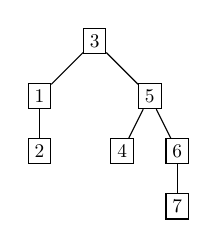
\begin{tikzpicture}[scale=0.7,level distance=10mm,level/.style={sibling distance=20mm/#1}]
	\tikzstyle{every node}=[draw,scale=0.7]
	\node (a){$3$}
	child {node (b) {$1$} child { node (c) {$2$} }}
	child {node (d) {$5$} child { node (e) {$4$} } child { node (f) {$6$} child { node (g) {$7$} } } };
\end{tikzpicture}
\end{minipage}
\vspace{0.5cm}

Die Schlüssel $s_i$ und $s_j$ werden also genau dann miteinander verglichen,
wenn nur $s_i$ oder $s_j$ als erstes aus $S_{ij} = \{ s_i, \dots, s_j \}$ als
Pivotelement gewählt werden:
\[
  X_{ij} = \begin{cases} 1 & \text{falls $s_j$-Knoten Nachfolger des
  $s_i$-Knoten oder umgekehrt} \\ 0 & \text{sonst} \end{cases}
\]
\begin{align*}
  \Rightarrow p_{ij} &= \Pr\left[s_i \text{ wird als erstes Pivotelement aus $S_{ij}$ gewählt}\right] \\
  &+ \Pr\left[s_j \text{ wird als erstes Pivotelement aus $S_{ij}$ gewählt}\right] = \frac{2}{j-i+1}
\end{align*}
Unter Verwendung der Eigenschaft der harmonischen Reihe $\ln(i+1) \leq H_i =
\sum_{k=1}^i \frac{1}{k} \leq 1 + \ln i$ ergibt sich für den Erwartungswert
\begin{align*}
	\sum_{i<j} p_{ij} &= \sum_{i=1}^n \sum_{j=1}^n \frac{2}{j-i+1} = 2 \cdot \sum_{i=2}^n \sum_{j=2}^i \frac{1}{j} \\
			  &\leq 2 \cdot \sum_{i=1}^n \left(H_i - 1\right) \leq 2 n \ln n = (2 \ln 2) n \log_2 n \approx 1.386\dots n \log_2 n
\end{align*}
\renewcommand\arraystretch{1.5}
\begin{tabular}{r|ccccccc}
	& & $j = 2$ & 3 & 4 & $\cdots$ & $n-1$ & $n$ \\
	\hline
	$i = 1$ & $0$ & $\frac{2}{2}$ & $\frac{2}{3}$ & $\frac{2}{4}$ & $\cdots$ & $\frac{2}{n-1}$ & $\frac{2}{n}$ \\
	$2$ && $0$ & $\frac{2}{2}$ & $\frac{2}{3}$ & $\cdots$ & $\cdots$ & $\frac{2}{n-1}$ \\
	$3$ &&& $0$ & $\frac{2}{2}$ & $\cdots$ & $\cdots$ & $\frac{2}{n-2}$
\end{tabular}

%%
\newpage

\ohead{12. Mai 2011}
\subsection{Ein \textit{Min-Cut}-Algorithmus}
\begin{defn}
	In einem Multigraphen kann es mehr als eine Kante zwischen zwei Knoten
	geben. Ein Schnitt in einem zusammenhängenden Multigraphen $G$ ist eine
	Kantenmenge, deren Entfernung aus $G$ den Multigraphen $G$ in zwei oder
	mehr Zusammenhangskomponenten zerlegt. Ein minimaler Schnitt
	(\emph{min cut}) ist ein Schnitt kleinstmöglicher
	Kardinalität\footnote{Das \emph{Max-Flow}-Problem ist zum
	\emph{Min-Cut}-Problem äquivalent}.
\end{defn}
\begin{exmp}
	Anwendung der Operation \emph{contract} auf einen einfachen Graphen.

	\vspace{0.5cm}
	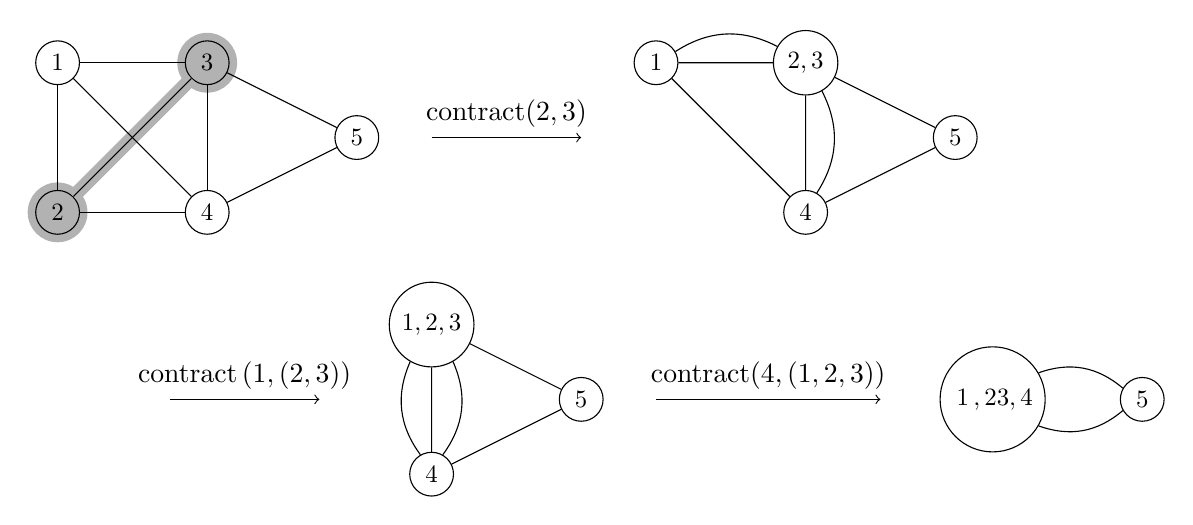
\begin{tikzpicture}[scale=0.95]
		\node[circle,draw,scale=0.9] (1) at (0,2) {$1$};
		\fill[black!30] (0,0) circle (0.40cm);
		\node[circle,draw,scale=0.9] (2) at (0,0) {$2$};
		\fill[black!30] (2,2) circle (0.40cm);
		\node[circle,draw,scale=0.9] (3) at (2,2) {$3$};
		\node[circle,draw,scale=0.9] (4) at (2,0) {$4$};
		\node[circle,draw,scale=0.9] (5) at (4,1) {$5$};
		\draw[line width=5pt,-,black!30] (2) -- (3);
		\draw (1) -- (2);
		\draw (1) -- (3);
		\draw (1) -- (4);
		\draw (2) -- (3);
		\draw (2) -- (4);
		\draw (3) -- (4);
		\draw (3) -- (5);
		\draw (4) -- (5);
		\draw[->] (5,1) to node[above] {$\textnormal{contract}(2,3)$} (7,1);
		\node[circle,draw,scale=0.9] (1b) at (8,2) {$1$};
		\node[circle,draw,scale=0.9] (23) at (10,2) {$2,3$};
		\node[circle,draw,scale=0.9] (4b) at (10,0) {$4$};
		\node[circle,draw,scale=0.9] (5b) at (12,1) {$5$};
		\draw (1b) -- (23);
		\path[draw] (1b) edge [bend left] (23);
		\draw (1b) -- (4b);
		\draw (23) -- (4b);
		\path[draw] (23) edge [bend left] (4b);
		\draw (23) -- (5b);
		\draw (4b) -- (5b);
		\draw[->] (1.5,-2.5) to node[above] {$\textnormal{contract}\left(1,(2,3)\right)$} (3.5,-2.5);
		\node[circle,draw,scale=0.9] (123) at (5,-1.5) {$1,2,3$};
		\node[circle,draw,scale=0.9] (4c) at (5,-3.5) {$4$};
		\node[circle,draw,scale=0.9] (5c) at (7,-2.5) {$5$};
		\draw (123) -- (4c);
		\draw (123) -- (5c);
		\draw (4c) -- (5c);
		\path[draw] (123) edge [bend left] (4c);
		\path[draw] (123) edge [bend right] (4c);
		\draw[->] (8,-2.5) to node[above] {\textnormal{contract}$\left(4,(1,2,3)\right)$} (11,-2.5);
		\node[circle,draw,scale=0.9] (1234) at (12.5,-2.5) {$\begin{matrix}1,2\\[-0.3cm]3,4\end{matrix}$};
		\node[circle,draw,scale=0.9] (5d) at (14.5,-2.5) {$5$};
		\path[draw] (1234) edge [bend left] (5d);
		\path[draw] (1234) edge [bend right] (5d);
	\end{tikzpicture}
\end{exmp}
\begin{defn}[Operation \emph{contract} einer Kante $\{x, y\}$]
	Ersetze $x$ und $y$ durch einen neuen Knoten $z$, lösche alle Kanten zwischen $x$ und $y$ und ersetze alle übrigen Kanten $\{x, v\}$ bzw. $\{y, v\}$ durch eine neue Kante $\{z, v\}$.
\end{defn}
\begin{algorithm}
	\caption{contract ($G$: Multigraph)}
	\vspace{0.4cm}
	\begin{enumerate}
		\setlength{\itemsep}{2pt}
		\setlength{\parskip}{2pt}
		\setlength{\parsep}{2pt}
		\item $H := G$
		\item \textbf{while} $H$ enthält mehr als $2$ Knoten \textbf{do}
		\item $\hphantom{while}$ wähle u.a.r.\ eine Kante $\{x, y\}$ aus $H$
		\item $\hphantom{while}$ contract$(x,y)$ in $H$
		\item[] \textbf{done}
		\item sei $C$ die Menge der Kanten in $H$ (rückgerechnet auf $G$)
		\item gib $C$ aus
	\end{enumerate}
\end{algorithm}
\subsubsection{Analyse der Erfolgswahrscheinlichkeit}
Sei $e_i$ die in der $i$-ten Iteration kontrahierte Kante, $1 \leq i \leq n-2$,
und sei $H_i$ der zugehörige Graph. $H_0 = G, H_{n-2}$ ist der letzte Graph.
\pagebreak
	\paragraph{Beobachtung 1:} Die Menge $C$ ist ein Schnitt von $H_0 = G$, da
		sie ein Schnitt von $H_{n-2}$ ist.\\[-0.75cm]
	\paragraph{Beobachtung 2:} In jedem Graphen $H_i$ ist die Größe eines
	\emph{min cuts} nicht kleiner als in $G$.\vspace{0.5cm}

Sei $K$ ein beliebiger \emph{min cut} in $G$. $K$ überlebt die Folge der
Kontraktionen genau dann, wenn keine der Kanten aus $K$ zur Kontraktion (in
jeder Iteration) ausgewählt wurde.
\[
  \Pr\left[C \text{ ist } min\ cut\right] \geq \Pr\left[C = K\right] = \Pr\left[
  \bigwedge_{1\leq i\leq n-2} \left(e_i \not\in K\right)\right] =
  \prod_{i=1}^{n-2} \Pr\left[e_i \not\in K\ \Big|\ \bigwedge_{1\leq j < i} \left(e_j
  \not\in K\right)\right]
\]

\begin{lemm}
	Für $1 \leq i \leq n-2$ gilt:
	\[ \Pr\left[e_i \in K | \bigwedge_{1\leq j < i} \left(e_j \not\in K\right) \right] \leq \frac{2}{n-i+1} \]
\end{lemm}
\begin{proof} Sei $k = |K|$ sowie $n = |V|$.
	\begin{itemize}
		\item Jeder Knoten des Eingabegraphen hat mindestens Grad $k$:
			\[ \frac{1}{2} \cdot |K| \cdot |V| \leq |E| \]
			Für die Wahrscheinlichkeit, dass im ersten Schritt eine
			der Kanten aus $K$ gewählt wird, gilt also
			\[ \Pr\left[e_1 \in K\right] \leq
			\frac{|K|}{\frac{1}{2}\cdot |K| \cdot |V|} =
			\frac{2}{n} \]
		\item $H_1$ hat $n-1$ Knoten, analog gilt also
			\[ \Pr\left[e_2 \in K\ |\ e_1 \not\in K\right] \leq
			\frac{|K|}{\frac{1}{2}\cdot |K| \cdot (n-1)} =
			\frac{2}{n-1} \]
		\item Für jedes $i$ mit $1 \leq i \leq n-2$ gilt somit die Ungleichung
			\[ \Pr\left[e_i \in K\ \Big|\ \bigwedge_{j=1}^{i-1}
			\left(e_j \not\in K\right)\right] \leq
			\frac{|K|}{\frac{1}{2}\cdot |K| \cdot
			\left(n-(i-1)\right)} = \frac{2}{n-i+1} \]
	\end{itemize}
\end{proof}

Damit lässt sich nun die Wahrscheinlichkeit abschätzen, dass $C$ (die Ausgabe
des \emph{contract}-Algorithmus) ein \emph{min cut} ist:
\[
  \Pr\left[ C \text{ ist } min\ cut\right] \geq \prod_{1\leq i \leq n-2}
  \left(1-\frac{2}{n-i+1}\right) = \prod_{i=1}^{n-2} \frac{n-i-1}{n-i+1} = \frac{2}{n(n-1)}
\]

\begin{satz}
	\emph{contract($G$)} gibt mit Wahrscheinlichkeit mindestens $\frac{2}{n(n-1)}$ einen \emph{min cut} aus.
\end{satz}

\subsubsection{Wahrscheinlichkeitsverstärkung (\emph{probability amplification})}
Wiederhole \emph{contract($G$)} $\frac{1}{2} \cdot c \cdot n(n-1)\cdot \ln n$
Mal (für beliebige Konstante $c$) und gib das beste $C$ aus.

Die Wahrscheinlichkeit, dass kein \emph{min cut} gefunden wurde, ist:
\[
  \left(1-\frac{2}{n(n-1)}\right)^{\frac{1}{2}c\,n(n-1)\,\ln n} \leq e^{-c\,\ln n} = \frac{1}{n^c}
\]

\subsection{Verifikation von Matrix-Produkten}
Gegeben: drei $n \times n$-Matrizen $A$, $B$, $C$ über $\{0, 1\}$ mit
Multiplikation und Addition modulo $2$.

Jemand behauptet: $A\cdot B = C$. Berechne $A\cdot B$ und teste auf Gleichheit.
Laufzeit\footnote{Coppersmith/Winograd: $\mathcal{O}(n^{2.376})$}
$\mathcal{O}(n^3)$.

\begin{algorithm}
	\caption{Algorithmus VerifyMatrixProduct}
	\vspace{0.4cm}
	\begin{enumerate}
		\setlength{\itemsep}{2pt}
		\setlength{\parskip}{2pt}
		\setlength{\parsep}{2pt}
		\item Wähle $v = \left(v_1, \dots, v_n\right)^T \in \{0, 1\}^n$ zufällig
		\item $u := B\cdot v$
		\item $w := A\cdot u$
		\item $x := C\cdot v$
		\item \textbf{if} $w \not= x$ \textbf{then return} \glqq sind ungleich\grqq
		\item[] \textbf{else return} \glqq sind gleich\grqq
	\end{enumerate}
\end{algorithm}

Der Algorithmus \emph{VerifyMatrixProduct} besitzt Laufzeit $\mathcal{O}(n^2)$,
was linearer Zeit entspricht, da die Eingabe bereits $\mathcal{O}(n^2)$ groß ist.

Wenn $A\cdot B = C$ ist, dann gilt
\[
  x = C \cdot v = \left( A \cdot B \right) v = A \left( B \cdot v \right) = A \cdot u = w
\]
Ist jedoch $A\cdot B \not= C$, so sei
\[
  D = A\cdot B - C
\]
und es gilt $D \not= 0$, d.h.\ es gibt mindestens ein $d_{i,j} \not= 0$. Sei $v
= \left( v_1, \dots, v_{j-1}, \ast, v{j+1}, \dots, v_n \right)^T \in \{0,
1\}^{n-1}$ beliebig, aber fest.
\[
  d_{i,1} \cdot v_1 + \dots + d_{i,j-1} \cdot v_{j-1} + d_{i,j} \cdot v_j +
  d_{i,j+1} v_{j+1} + \dots + d_{i,n} \cdot v_n = 0
\]
Dies ist eine Gleichung, die nach $v_j$ aufgelöst werden kann (da $d_{i,j}
\not= 0$) und damit genau eine Lösung hat. Der Algorithmus hat zwei
Möglichkeiten zur Wahl von $v_j$.
\[
  \Pr\left[ A\cdot B \cdot v = C \cdot v \right] = \Pr\left[ \left(A\cdot B -
  C\right) v = 0 \right] = \Pr\left[ D \cdot v = 0 \right] \leq \frac{1}{2}
\]

Dies bedeutet, dass eine unerwünschte Ausgabe von \glqq sind gleich\grqq mit
Wahrscheinlichkeit kleiner $\frac{1}{2}$ auftritt (bei Gleichheit wird immer
korrekt \glqq sind gleich\grqq\ ausgegeben). Nach $c$-maliger Ausführung des
Algorithmus gilt
\[
  \Pr\left[ \text{$c$-fache Wiederholung zeigt nicht $A\cdot B \not= C$}
  \right] \leq \left(\frac{1}{2}\right)^c
\]
